\subsection{Benchmarking instances}

This section explains the two sets of benchmarks used for testing the ILP, GRASP and BRKGA models. First we discuss about how the size of a problem instance can be determined. Then we show how we created two sets of problems instances, the medium size data set consisting of 38 small or medium size instances, and the large size data set consisting of 200 problem instances. The medium size set is used to compare the ILP model versus the Metaheuristics models. The large size set is used to test parameter values in order to find the best performing setup for each BRKGA and GRASP model, and finally to compare them solving one large problem instance.


\subsubsection{The instance generation process}

The algorithm used for generate problem instances is based on generating random but valid schedules of nurses and then extracting the demand for each schedule. This approach assures that the problem instance will always have a solution.

The algorithm takes as input: the number of nurses, the proportion of extra nurses to add to the minimum needed to solve the problem, the hours of the schedule and the rest of the constraints of the schedules (max hours, min hours, max presence and max consecutive hours). It then generates 2 types of schedules, one that concentrates the working hours as much as the constraints allow it to, and another one with as much alternated rest hours and working hours as the constraints permit it. Then the algorithm can choose to place the generated schedules around selected hours (the algorithm can choose one, two, three or four different hours to start working schedules at). We add some variability on the exact hour at which each schedule starts around the selected hours. Once all schedules are placed, the number of working nurses for each our is added and the demand for each hour is then computed.


\subsubsection{The medium and large sets}

To decide how the size of a problem is determined, we choose to reference the time it takes for the ILP model to solve the problem instance using the Cplex solver. We generate and solve a series of instances with the ILP until we have around 20 instances that take 60 minutes or less to solve by ILP. Then, as we cannot perform the same procedure to generate the large size set, we execute a series of experiments to determine the influence of the problem variables in the time it takes for the ILP model to solve it.\\

The next figures show different executions of a small modification of a problem instance. In each figure, a parameter of the problem is modified and that modifies the number of steps the ILP model has to do to decrease the gap between the best integer and the best bound until a gap of 0.05 is reached. The number of steps is then an indication of the time it takes to solve the problem, and thus it gives us an idea of what parameters increase do the size of the problem instance.\\


\begin{figure}[h!]

\begin{subfigure}[b]{.49\linewidth}
\centering
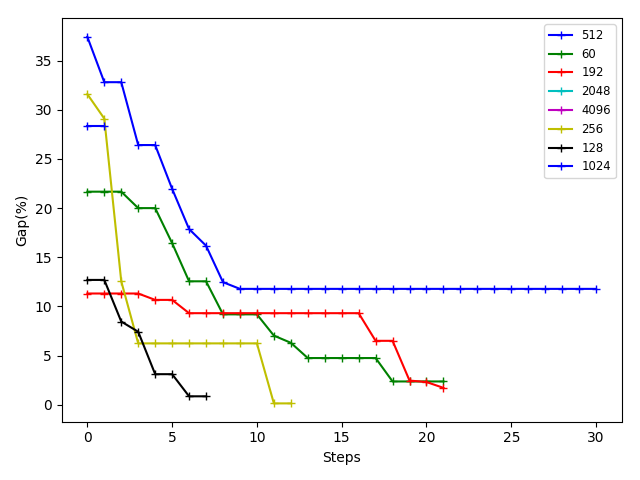
\includegraphics[width=\linewidth]{./img/instances_nurses_ilp_evol.png}
\caption{ Evolution of Gap of the ILP model with different number of nurses}\label{fig1a}
\end{subfigure}%
\begin{subfigure}[b]{.49\linewidth}
\centering
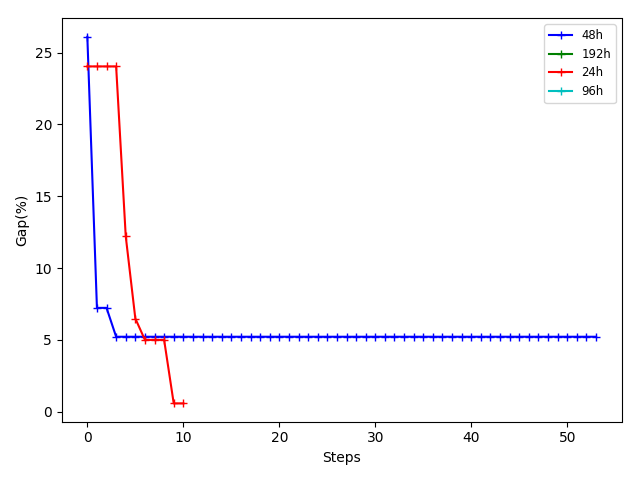
\includegraphics[width=\linewidth]{./img/instances_hours_ilp_evol.png}
\caption{ Evolution of Gap of the ILP model with different number of hours }\label{fig1b}
\end{subfigure}\vfill
\caption{Evolution of Gap of the ILP model with different values of number of nurses (\subref{fig1a}) and number of hours (\subref{fig1b}). }
\label{fig_ilp_size}
\end{figure}


\begin{figure}[h!]
\begin{subfigure}[b]{.49\linewidth}
\centering
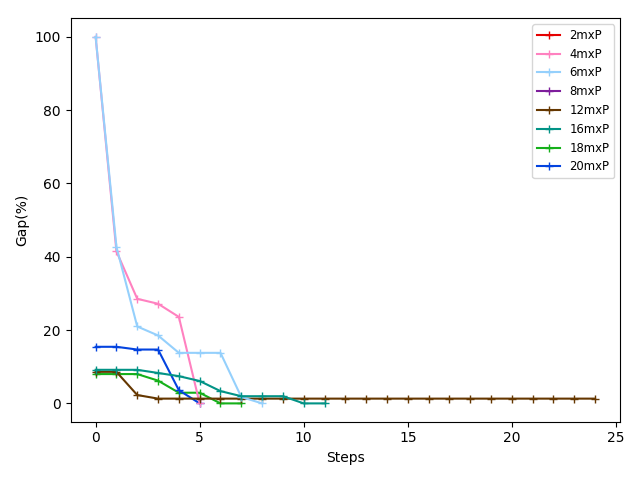
\includegraphics[width=\linewidth]{./img/instances_maxpresence_ilp_evol.png}
\caption{Evolution of Gap of the ILP model with different values of maxPresence parameter }\label{fig1c}
\end{subfigure}
\begin{subfigure}[b]{.49\linewidth}
\centering
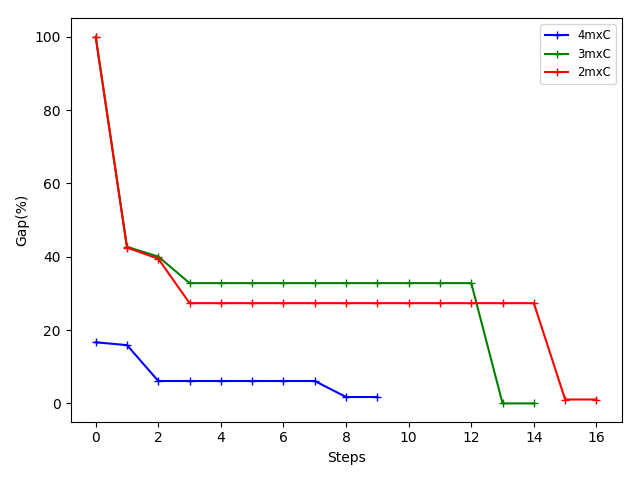
\includegraphics[width=\linewidth]{./img/instances_maxconsec_ilp_evol.png}
\caption{Evolution of Gap of the ILP model with different values of maxConsec parameter }\label{fig1d}
\end{subfigure}
\caption{Evolution of Gap of the ILP model with different values of maxPresence (\subref{fig1c}) and maxConsec (\subref{fig1d}).  }
\label{fig_ilp_size2}
\end{figure}


\begin{figure}[h!]
\begin{subfigure}[b]{.49\linewidth}
\centering
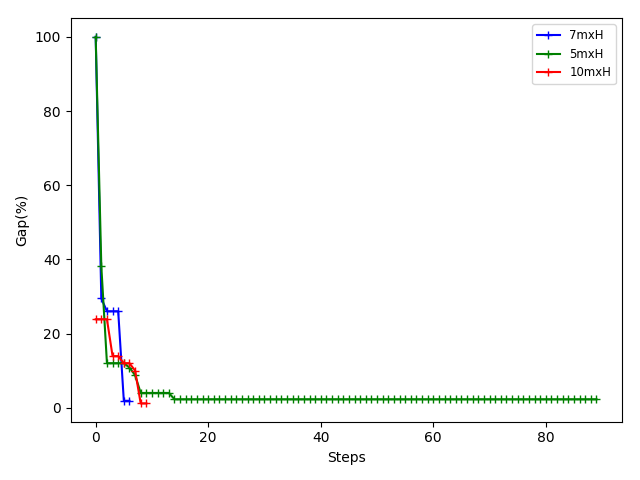
\includegraphics[width=\linewidth]{./img/instances_maxhours_ilp_evol.png}
\caption{Evolution of Gap of the ILP model with different values of maxHours parameter }\label{fig1c}
\end{subfigure}
\begin{subfigure}[b]{.49\linewidth}
\centering
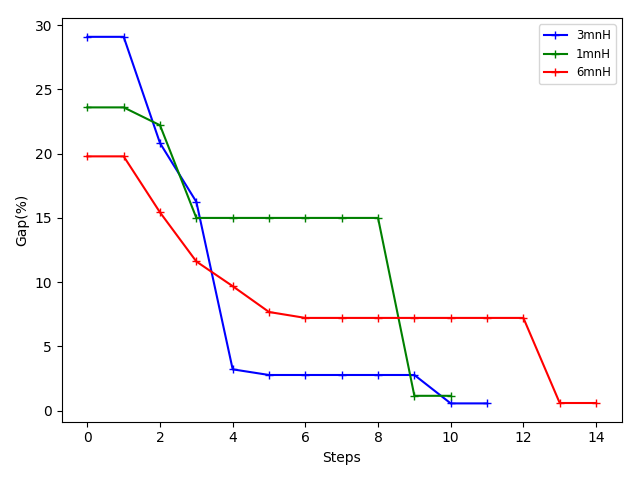
\includegraphics[width=\linewidth]{./img/instances_minhours_ilp_evol.png}
\caption{Evolution of Gap of the ILP model with different values of minHours parameter }\label{fig1d}
\end{subfigure}
\caption{Evolution of Gap of the ILP model with different values of maxHours (\subref{fig1c}) and minHours (\subref{fig1d}).  }
\label{fig_ilp_size3}
\end{figure}


The results in figure~\ref{fig_ilp_size}, figure~\ref{fig_ilp_size2} and figure~\ref{fig_ilp_size3} page~\pageref{fig_ilp_size} allow us to conclude how the parameters of the problem instance can be modified to increase its solving time and thus what we consider its size. The large set of problem instances will be generated using modifications of those instance variables, applied to some problems of the medium size set. The table~\ref{tab:ilp_size} page~\pageref{tab:ilp_size} summarizes the findings and shows the attributes of each benchmark instance set.

\begin{table}[ht] 
\centering 
\begin{tabularx}{0.75\textwidth}{|l|c|c|c|}
\hline
\textbf{Problem} & \textbf{Effect on problem size}  & \textbf{Medium size set} & \textbf{Large size set} \\

\textbf{Variable}  		& \textbf{when increasing}  & 38 instances &  199 instances \\
\hline
\textbf{$nNurses$} & increases      &  64	&  64 to 1600 \\
\textbf{$hour$}   & increases		& 24	&  24, 48, 72 \\
\textbf{$maxPrensce$} & decreases	& 16	& 8 to 27 \\
\textbf{$maxConsec$} & decreases		& 5	&  4 to 13		\\
\textbf{$maxHours$} & decreases		& 4 to 10	& 2 to 12 \\
\textbf{$minHours$} & increases		& 1 to 5	& 1 to 9\\
\hline
\end{tabularx}
\caption{Benchmark datasets and variables influence on problem size}
\label{tab:ilp_size}
\end{table}


